\section{Offline Computation}
The offline computation of selective decoding retrieves the dependencies by partially decoding a video. It is essential to understand various dependencies in order to comprehend offline computation. For all subsequent discussions in this paper, we assume the video is in YCbCr420 color space, which means a macroblock contains four luminance blocks and two chrominance blocks.  
\subsection{Dependencies}
Two categories of dependencies can be identified, namely intra-frame dependency and inter-frame dependency. Dependencies are the reason why some macroblocks outside of ROI need to be decoded. By saving certain information, we can reduce the dependencies and improve the efficiency of selective decoding. Below we analyze the dependencies and introduce the methods to reduce them. 
\subsubsection{Intra-frame Dependency}
Intra-frame dependency refers to the dependencies among macroblocks within a single frame. There are two sources of intra-frame dependency, including DC\&AC Prediction and MV coding. 

DC\&AC Prediction is performed for I-macroblock when the header field short\_video\_header is set to '0'. It consists of two steps, namely reference block selection and prediction decoding. The reference block selection step can be illustrated by Fig 2.

\begin{figure}
\centering 
%\vspace{2.5cm}
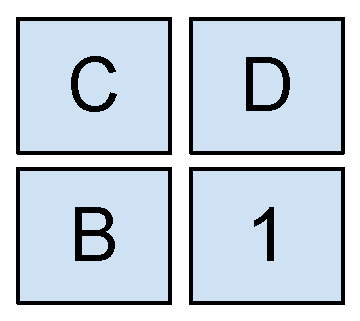
\includegraphics[height=1.2cm]{pred.eps}
\caption{DC\&AC Prediction Reference Block Selection}
\end{figure}
There are two candidate reference blocks for each block, the immediate left block and the immediate upper block. In addition, the upper left block is also needed in order to determine the reference block. To determine the reference block for block 1 in Fig 2, the following rule is applied,
%\begin{verbatim} 
{\tt \\if (|F(B)[0][0] - F(C)[0][0]| < |F(C)[0][0] - F(D)[0][0]|)\\
\indent predict from block D \\
else  \\
\indent predict from block B \\} 
%\end{verbatim}
F(B)[0][0], F(C)[0][0] and F(D)[0][0] refer to inverse quantized DC value of block B, C and D respectively. The selection rule indicates one block is dependent on three neighboring blocks. In the actual prediction decoding, the decoding block depends only on the selected reference block.

Two out of three blocks are only needed to determine the prediction direction, which is either up or left. A single bit is enough to record this information, with '0' indicating up and '1' referring to left. This reduces the dependency for a block from three to one.

MV of P-frame is differentially coded, which is the other source of intra-frame dependency. At motion decoding, the decoder recovers the MV values based on the decoded base values and residue values obtained from neighboring macroblocks. In selective decoding, the MVs are recorded to trace the Inter-frame Dependency, which is discussed next. Therefore the MVs can be read directly by decoder and no MV prediction decoding is needed. Thus the dependency due to MV prediction decoding is eliminated completely.
  
\subsubsection{Inter-frame Dependency}
Inter-frame dependency refers to the dependencies among macroblocks at different frames, which is caused by motion compensation coding. In MPEG4 SP, motion compensation decoding only occurs at P-macroblock of P-frame. The inter-frame dependency is illustrated as Fig 3.

\begin{figure}
\centering
%\vspace{2.5cm}
%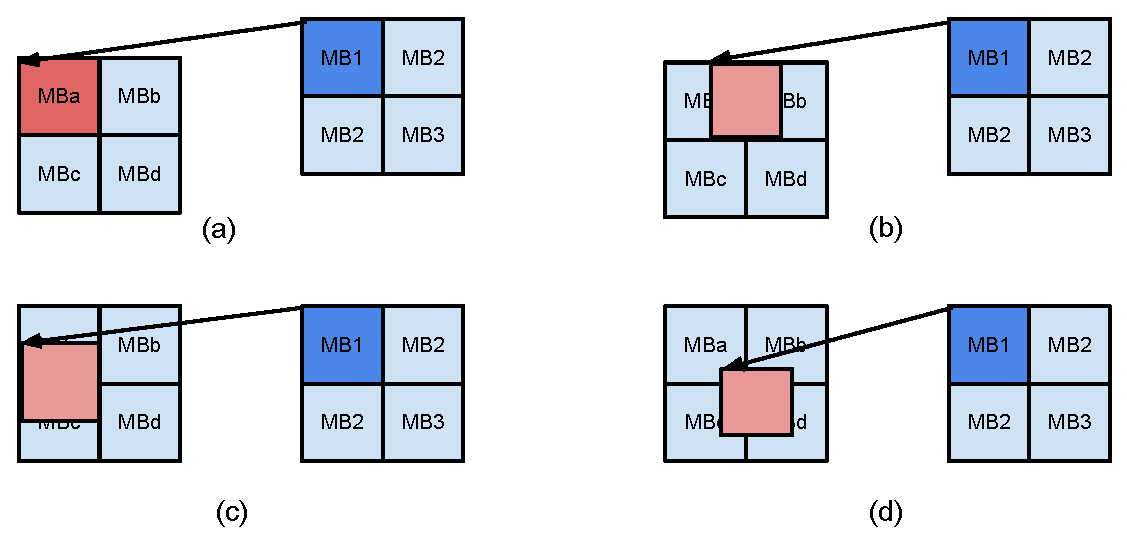
\includegraphics[height=2.5cm]{mm1.eps}
\subfigure[]{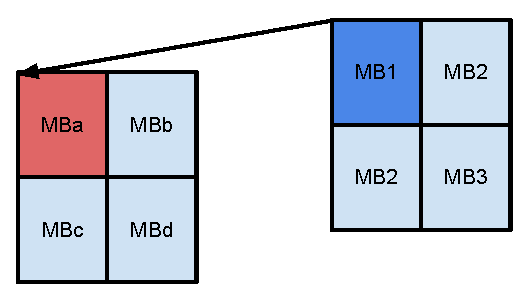
\includegraphics[height=1.15cm]{me1.eps}}
\quad
\subfigure[]{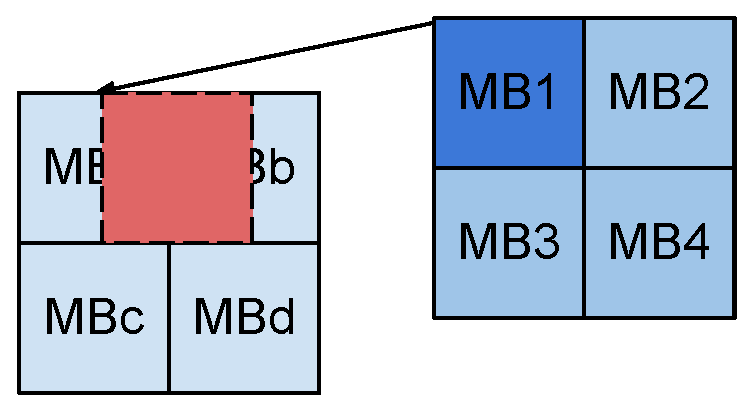
\includegraphics[height=1.15cm]{me2.eps}}
\quad
\subfigure[]{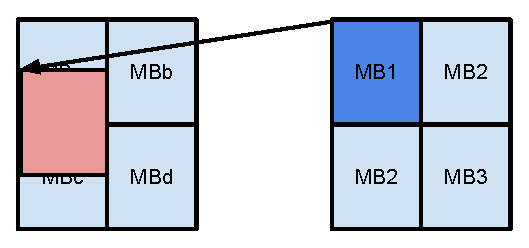
\includegraphics[height=1.15cm]{me3.eps}}
\quad
\subfigure[]{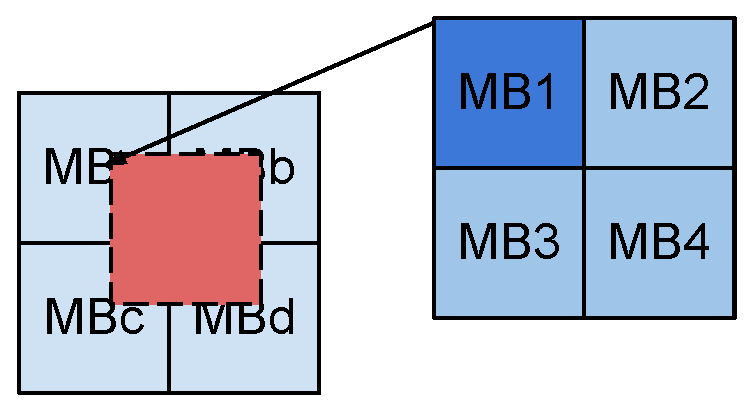
\includegraphics[height=1.15cm]{me4.eps}}
\caption{Different Cases of Motion Compensation Decoding}
\end{figure}
Motion compensation decoding is performed on MB1 of the current frame, with reference to a region of a previous frame. The number of dependent macroblocks depends on whether the reference region aligns with the macroblock boundary. As shown in Fig 3, MB 1 depends on one macroblock at (a), two macroblocks at (b) and (c), and four macroblocks at (d). 

Khiem etc. proposed an approach to reduce dependency due to motion compensation\cite{Ngo:2011:AEZ:1943552.1943581}. We adopted their technique in this research. Using the case in Fig 3(d) as an example, the approach is illustrated Fig 4.

\begin{figure}
\centering
%\vspace{2.5cm}
%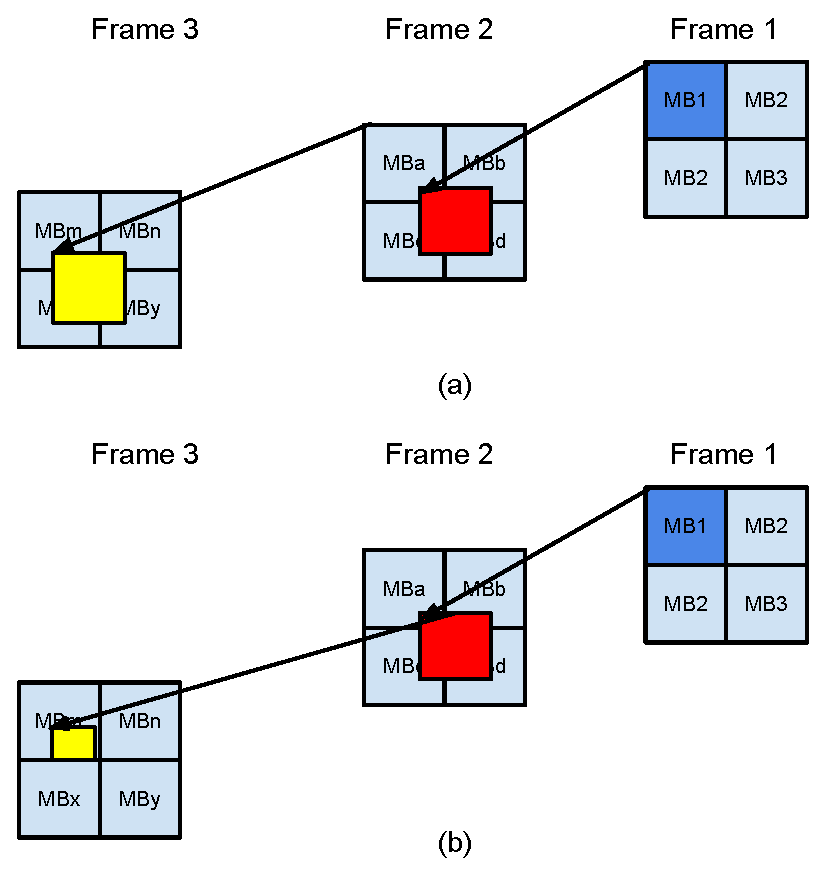
\includegraphics[height=2.5cm]{mm2.eps}
\subfigure[]{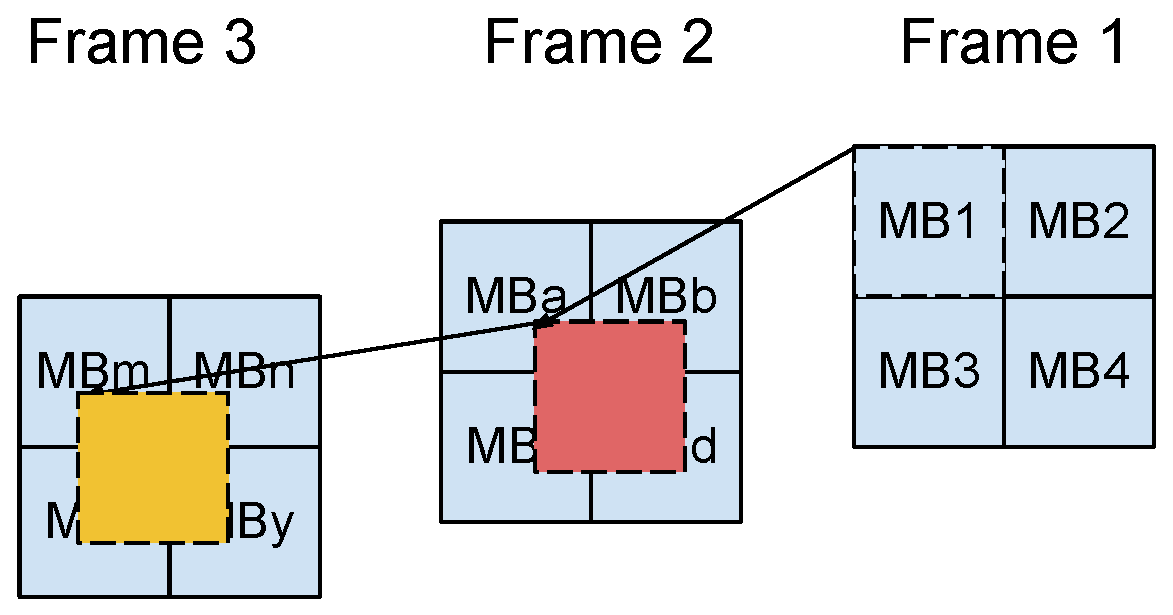
\includegraphics[height=2.0cm]{meo1.eps}}
\quad\quad
\subfigure[]{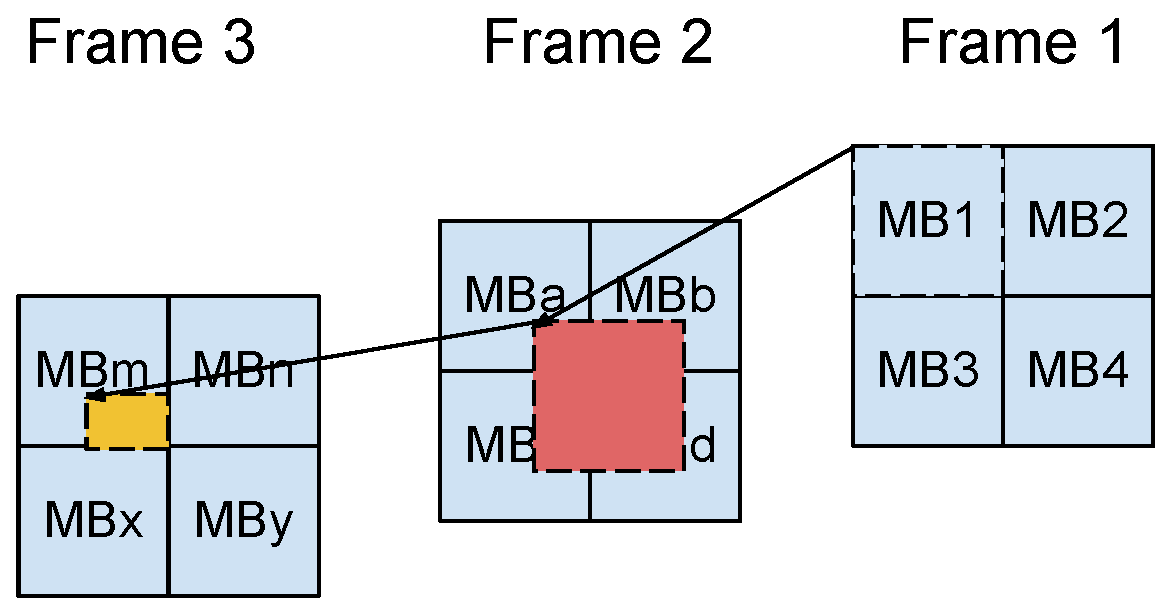
\includegraphics[height=2.0cm]{meo2.eps}}
\caption{Dependency Analysis for Motion Compensation}
\end{figure}

MB1 at Frame 1 depends on four macroblocks at Frame 2. MBa at Frame 2 depends on another four macroblocks at Frame 3. Dependency can be reduced by tracing it at pixel level. The dependency between Frame 1 and Frame 2 remains the same. But we do not really need all pixels at Frame 2 MBa. The region needed at MBa depends on only part of MBm at Frame 3. Therefore, the dependency for MBa between Frame 2 and 3 are reduced from four to one in this example.

\subsection{Dependency Files}
The offline computation partially decodes a video and records down the dependency information into a set of files named dependency files. The dependency files are generated for each Group of VOP (GOP). For every GOP, the dependency files include the following,
\begin{enumerate}
\item GOP record file: this file contains the start and end frame numbers of a GOP. 
\item MB start and end position file: this file stores the macroblock start and end bit positions in the video bitstream for every MB of all frames in the GOP. The start and end positions are needed for the decoder to seek the bits for a macroblock. 
\item DC\&AC Prediction direction file: this file contains the DC\&AC Prediction direction. A single bit is used to store the direction for each block. The direction is read directly by the decoder to avoid decoding the macroblocks used in DC\&AC Prediction reference selection but not in actual prediction decoding. The direction is also used to trace the intra frame dependency.  
\item MV file: this file records the MV values for every macroblock of each P-frame in the GOP and the number of bits for MVs. The selective decoder reads the MV from this file and skip the encoded bits. This file does not only eliminate the MV decoding dependency, but also allows the online computation to trace the inter-frame dependency.
\end{enumerate}
We modified the standard MPEG4 SP decoder to partially decode a video in order to generate the above files. 

 



